\chapter{Simulation}\label{chap:sim}
	The data collected by the ATLAS experiment must be compared to a control. This control is most often a dataset of simulation particle collisions that approximate to great precision physics processes and particle interaction with detector material, as well as the detector's response. Figure \ref{fig:simulation} shows the chain of simulations these datasets are produced by. 
	\begin{figure}[!ht]
	\centering
	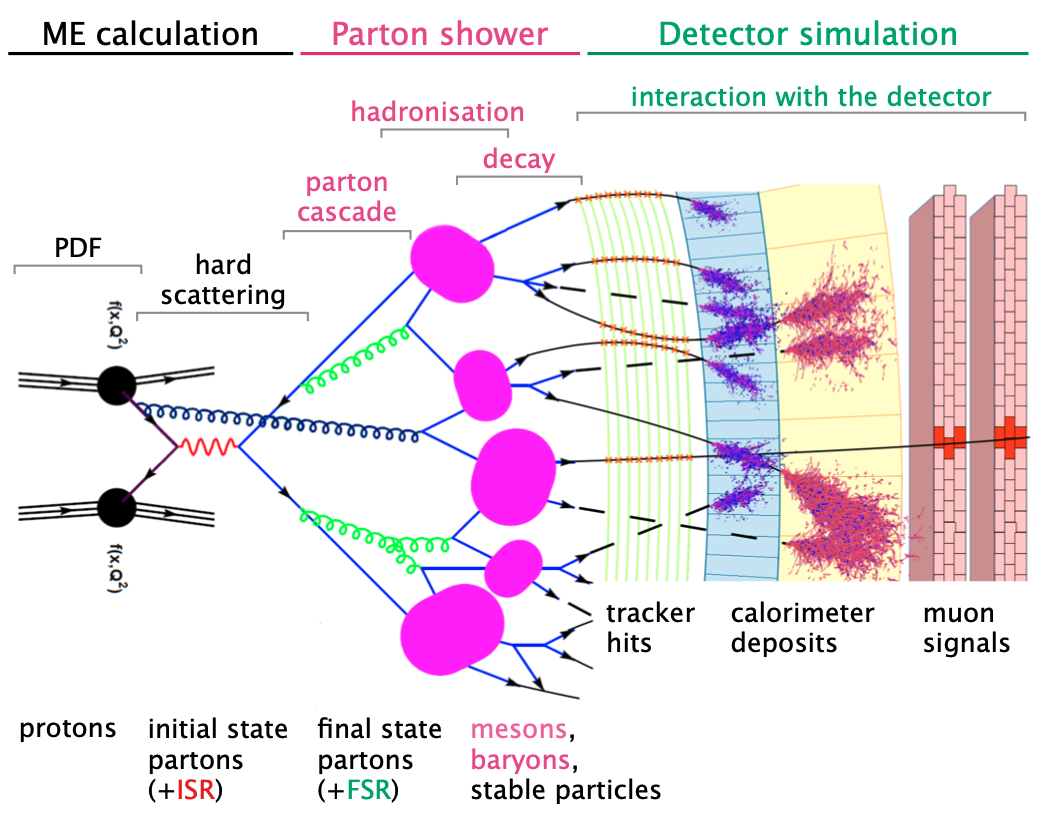
\includegraphics[width=.95\textwidth,keepaspectratio=true]{chapters/chapter4_simulation/images/Simulation_Chain.png}
	\caption{\label{fig:simulation} A pictorial representation of the simulation chain used in the ATLAS experiment. \cite{Wanotayaroj:2242196}}
	\end{figure}
	
	Many particle physics experiments, ATLAS included, use Monte Carlo (MC) simulation techniques to produce these datasets. Monte Carlo simulation techniques use repeated random sampling of underlying probability density functions to closely model various processes. 

	\section{Event Generation and Hadronization}\label{sec:event-gen}
	Since protons and other hadrons are not fundamental particles, it is impossible to know the exact constituents (partons) that interacted during a collision. To mimic this intrinsic probabilistic nature, Parton Distribution Functions (PDFs) are used. Where a PDF models the probability of any parton within a proton (or hadron) to carry a fraction of the beam energy as momentum. The PDF and subsequent inelastic hard scattering of the interacting partons are modeled via a Matrix Element (ME) calculation, often depicted through Feynman diagrams. This ME calculation is done to fixed order in perturbation theory, leading order (LO), next-to-leading order (NLO), leading-logarithmic order (LL), etc. This first level event generation can be done by a myriad of MC event generators. Often specific choices are made based on individual generator performance for a given physics process.

	The next step in the simulation chain is the parton showering or hadronization. This is often done with a completely different set of MC generators. Hadronization is a complex, computationally expensive step to simulate and is done through iteratively. An example of a parton shower generator output can be seen in figure \ref{fig:hadronization}.

	\begin{figure}[!ht]
	\centering
	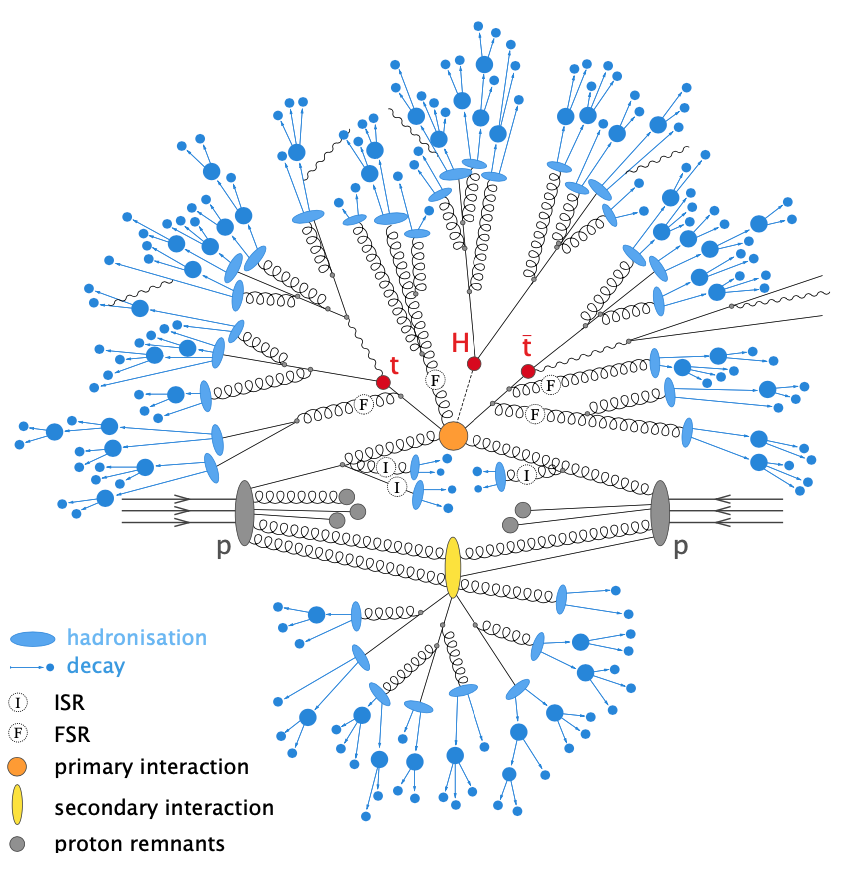
\includegraphics[width=.65\textwidth,keepaspectratio=true]{chapters/chapter4_simulation/images/tth_hadronization_gen.png}
	\caption{\label{fig:hadronization} A pictorial representation of a parton shower of a ttH event. \cite{Wanotayaroj:2242196}}
	\end{figure}	

	\section{Detector Simulation}\label{sec:detector-sim}
	The final step in the simulation chain is simulating the particle's interaction with the detector material and the detector's response. Up until this point, the MC generators used are generic non-experiment dependent simulations. The ATLAS collaboration uses a GEANT4 based generator suite to simulate these interactions. \cite{GEANT4} These simulations are incredibly detailed, including all support structure, material densities, readout electronics, digitization, etc. The final simulated dataset is output into a raw data format identical to real data coming off of the ATLAS detector.